% ================= APPENDIX: ELECTRICAL SYSTEM DETAIL =================
\section{Electrical System Detail}
\label{app:electrical}

This appendix holds the electrical detail kept out of
Section~\ref{sec:electrical}: the full schematic capture, the connector and pin
assignments, the harness drawings, the board layout and the bring-up
checklists. The architectural decisions --- two rails behind one E-stop, linear
bus topology, perfboard rather than fabricated board --- remain in
Section~\ref{sec:electrical}. The part specifications are in
Appendix~\ref{app:bom} and are not repeated.

\subsection{Schematic Capture}
\label{app:schematics}
\label{app:schematic_full}

The system is captured on one flat KiCad sheet, reproduced at page size in
Figure~\ref{fig:schematic_full} and listed by functional block in
Table~\ref{tab:schematic_sheets}. That capture is the working drawing the build
is wired from. The blocks it carries are: power entry and protection (pack
connector, anti-spark inrush path, combined E-stop and fuse, split to the motor
bus and the logic rail); the \qty{5}{\volt} logic rail off an LM2596 converter
with back-feed protection and per-device decoupling; the CAN-FD bus as a linear
chain across the three moteus drivers and the flight computer, terminated at
the two physical ends only; the per-axis encoder SPI interfaces; the Teensy 4.1
flight computer with the BMI270 IMU; the ESP32 telemetry link; and the three
brake servo drives.

Note: the MA600 breakout is paired with a diametric ring magnet
(\qty{4}{\milli\metre} thick; Appendix~\ref{app:bom}). The datasheet-recommended
air gap for the \qty{20}{\milli\tesla}--\qty{80}{\milli\tesla} nominal magnetic
field window is \qty{2}{\milli\metre}; the gap set on the build, and used
throughout this document, is \qty{1.5}{\milli\metre}.

Each block of the capture is checked against its own layout, mounting and
connection constraint before bring-up. That constraint table
(Table~\ref{tab:schematic_sheets}) is given in Section~\ref{sec:components},
ahead of the schematic itself, and is not repeated here. Component current
ratings are given in Appendix~\ref{app:electrical_ratings}
(Table~\ref{tab:electrical_ratings}).

\subsection{Component Current Ratings}
\label{app:electrical_ratings}

Table~\ref{tab:electrical_ratings} states the current each component on the
\qty{5}{\volt} logic rail and the pack rail is rated to draw. It replaces a
measured-consumption table: at this stage no bench data exists, and a table of
data\-sheet ratings is a stronger design input than an empty one, since the
\qty{5}{\volt} rail is sized against the coincident worst case --- telemetry
transmit burst, servo stall and full sensor load at once --- and not the sum
of typical values. Two entries are marked as unavailable rather than
estimated: neither manufacturer publishes a stall or supply-current figure for
that part, and a fabricated number would be worse than an honest gap. Both are
closed by the bench measurement of Table~\ref{tab:electrical_measured} during
electrical bring-up (Section~\ref{sec:electrical_safety}).

\begin{table}[htbp]
\centering
\caption[Component current ratings]{Component current ratings, by rail. Datasheet figures where
published; measured values replace these per Table~\ref{tab:electrical_measured}.}
\label{tab:electrical_ratings}
\small
\setlength{\tabcolsep}{4pt}
\begin{tabular}{L{3.4cm} c L{2.6cm} L{5.2cm}}
\toprule
Component & Rail & Rated current & Basis \\
\midrule
Teensy 4.1 & \qty{5}{\volt} & ${\approx}\,\qty{100}{\milli\ampere}$ & Board only, \qty{600}{\mega\hertz}, no shields (PJRC community data) \\
XIAO ESP32-C6 telemetry & \qty{5}{\volt} & ${\approx}\,\qty{300}{\milli\ampere}$ & TX burst (Table~\ref{tab:bom-supplied}) \\
BMI270 IMU & \qty{5}{\volt} & ${\approx}\,\qty{0.7}{\milli\ampere}$ & Typical, full \qty{6.4}{\kilo\hertz} ODR (Bosch datasheet) \\
MG92B brake servo (each, $3\times$) & \qty{5}{\volt} & \textcolor{red}{Not published} & TowerPro does not publish a stall-current figure; measure during bring-up \\
MA600 encoder (each, $3\times$) & \qty{5}{\volt} & \textcolor{red}{Not published} & MPS datasheet does not state supply current in the accessible electrical table; measure during bring-up \\
moteus-n1 driver (each, $3\times$) & Pack & \qty{100}{\ampere} peak / \qty{9}{\ampere} cont. & Datasheet (Table~\ref{tab:bom-supplied}) \\
MN4006 motor (each, $3\times$, via driver) & Pack & \qty{16}{\ampere} peak, thermally limited & Manufacturer bench data (Sec.~\ref{sec:architecture}) \\
\bottomrule
\end{tabular}
\end{table}

% The full schematic is drawn on its own landscape page rather than scaled into
% the text block: reduced to \textwidth in portrait the reference designators
% and net labels fall below legibility. Same treatment as the Gantt sheets of
% Sec. 3 -- see sections/02_project_organization_gantt.tex.
%
% Source: images/schematic_full.pdf, a single-page A4 landscape vector export
% from KiCad (a copy of "Cubli Schematic Right.pdf", renamed because
% \includegraphics does not take spaces in a path). Re-export over that file to
% update the sheet; no edit here is needed. On a landscape page \linewidth is the
% long edge, so the height limit is expressed in \textwidth -- with
% keepaspectratio, whichever bound binds first is the one applied.

% Empty page style for the rotated sheet: the running header and footer would
% otherwise be typeset sideways along the page edge.
\fancypagestyle{cublischematic}{%
  \fancyhf{}%
  \renewcommand{\headrulewidth}{0pt}%
  \renewcommand{\footrulewidth}{0pt}%
}

\begin{landscape}
\pagestyle{cublischematic}
\begin{figure}[p]
\thispagestyle{cublischematic}
\centering
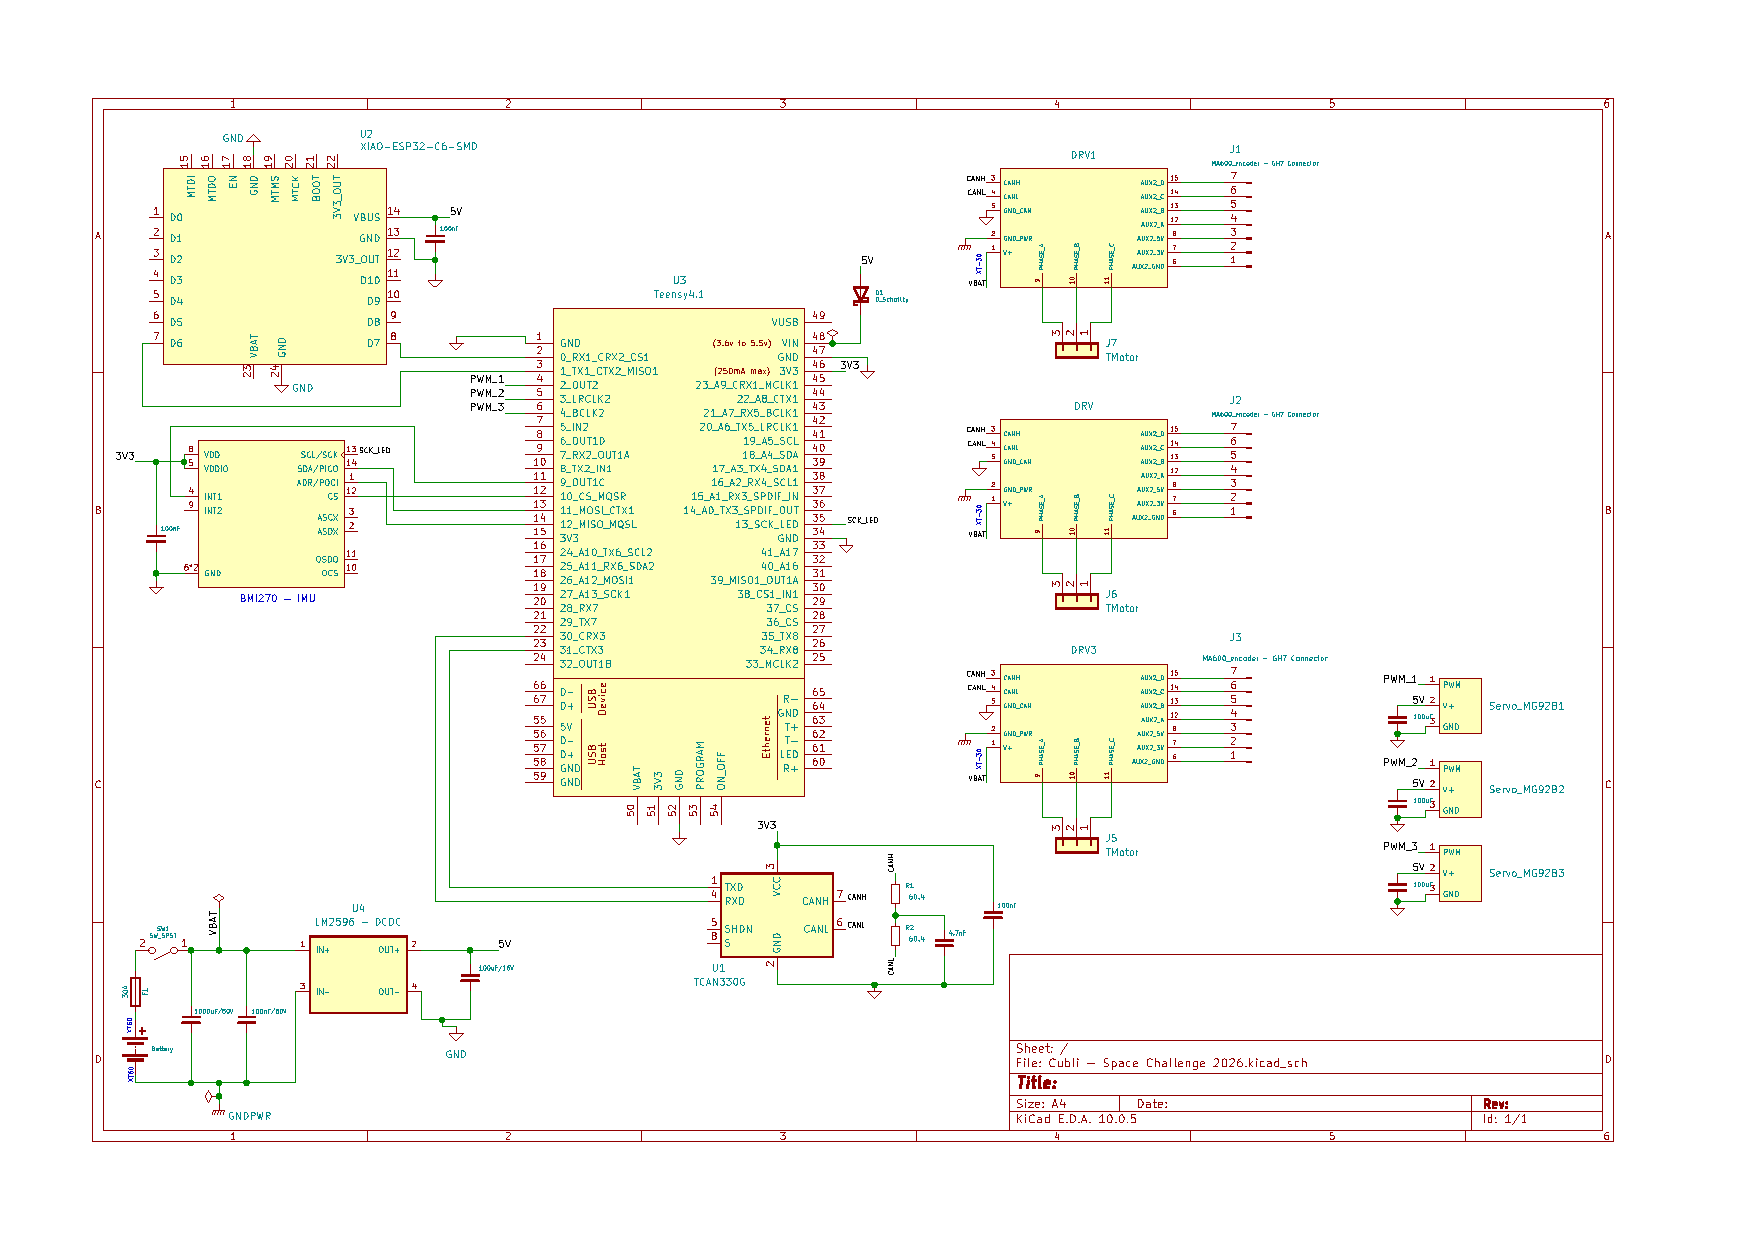
\includegraphics[width=\linewidth,height=1.0\textwidth,keepaspectratio]{images/schematic_full.pdf}
\caption[Full electrical schematic (landscape sheet)]{Full electrical schematic as captured, reproduced at page size.
Covers the flight computer (Teensy 4.1) and its ESP32 telemetry module, the
BMI270 IMU, the three moteus driver and motor connectors, the CAN-FD
transceiver and termination, the LM2596 \qty{5}{\volt} converter from the pack,
and the three brake servos.}
\label{fig:schematic_full}
\end{figure}
\end{landscape}
\pagestyle{fancy}

\subsection{Connector and Pin Assignments}
\label{app:pinout}

Table~\ref{tab:connectors} is the connector schedule. It exists so that a
harness can be built and re-built from this document alone, and so that a
mis-mate is a documented impossibility rather than a discovered one: no two
connectors carrying different voltages share a housing type on this machine.

\begin{table}[htbp]
\centering
\caption[Connector schedule]{Connector schedule. Keying and housing types are chosen so that two
connectors carrying different voltages cannot be mated. Note: values have not been finalized at this preliminary stage. }
\label{tab:connectors}
\small
\setlength{\tabcolsep}{4pt}
\begin{tabular}{c L{3.0cm} L{3.0cm} L{2.4cm} L{3.2cm}}
\toprule
Ref & From & To & Signals \\
\midrule
J1 & Battery pack        & Protection / E-stop   & \textcolor{red}{TBD} & Pack $+$, pack $-$ \\
J2 & Protection          & Distribution board    & \textcolor{red}{TBD} & Motor bus \\
J3 & Distribution board  & Driver, axis 1        & \textcolor{red}{TBD} & Motor bus \\
J4 & Distribution board  & Driver, axis 2        & \textcolor{red}{TBD} & Motor bus \\
J5 & Distribution board  & Driver, axis 3        & \textcolor{red}{TBD} & Motor bus \\
J6 & Board               & CAN chain, end A      & \textcolor{red}{TBD} & CAN-H, CAN-L, GND \\
J7 & CAN chain, end B    & Termination network   & \textcolor{red}{TBD} & CAN-H, CAN-L, GND \\
J8 & Driver, axis $i$    & Encoder, axis $i$     & \textcolor{red}{TBD} & SPI, \qty{3.3}{\volt}, GND \\
J9 & Board               & IMU                   & \textcolor{red}{TBD} & Serial bus, supply, GND \\
J10 & Board              & Telemetry module      & \textcolor{red}{TBD} & UART, supply, GND \\
J11 & Board              & Brake servo, axis $i$ & \textcolor{red}{TBD} & PWM, \qty{5}{\volt}, GND \\
\bottomrule
\end{tabular}
\end{table}

\subsection{Harness Drawings and Wire Schedule}
\label{app:harness}

The harness is organised into seven runs: pack to protection, protection to
board, board to the three driver drops, the three motor phase leads, the CAN
chain segments, the three encoder SPI runs, and the three servo drives. Wire
gauge on the motor bus (pack-to-protection, protection-to-board, driver drops
and motor phase leads) is sized on spin-up current rather than the balancing
current, since spin-up is the sustained high-current phase; the CAN and
encoder SPI runs are sized on length limits rather than current
(Table~\ref{tab:schematic_sheets}); the servo drives are sized on stall current.
Gauge and run length are recorded once measured on the assembled harness.

% Figure placeholder: distribution harness drawing -- pack lead, protection
% element, and the three driver drops, with labelling scheme.
% Figure placeholder: as-built harness photograph, labelled and strain-relieved.

\subsection{Board Layout}
\label{app:board_layout}

% Figure placeholder: perfboard floorplan -- bus entry, converter, logic rail,
% bulk capacitance, flight computer, IMU, telemetry module, servo headers and
% the CAN termination network.
% Figure placeholder: board outline drawing with the mounting-hole pattern,
% keep-out heights and connector exit directions delivered to the mechanical
% design as the electronics-mount interface of Table~\ref{tab:mech_interfaces}.

The floorplan is constrained before it is aesthetic: the driver positions follow
from the encoder cable limit, the bus route follows from the driver positions,
and the board is placed around what remains
(Section~\ref{sec:bus_topology}). Rail separation is maintained physically on
the board, not only schematically, so that motor-current return does not share
copper with the sensing ground.

\subsection{Bring-Up and Isolation Checklists}
\label{app:checklists}

These checks are performed on every re-assembly, not only on first build, since
the encoder gaps and connector seating are exactly what mechanical work
disturbs.

\paragraph{Before any power is applied.}
\begin{enumerate}
  \item Isolation: motor bus to chassis, logic rail to motor bus, each rail to
        ground.
  \item Capacitor voltage ratings confirmed by position --- no low-voltage part
        on the pack bus.
  \item Polarity of every fabricated connector verified against
        Table~\ref{tab:connectors}.
  \item Protection element in circuit: E-stop functional, fuse fitted and rated,
        anti-spark path intact.
  \item Encoder air gaps re-measured after mechanical assembly.
\end{enumerate}

\paragraph{First power-on, current-limited bench supply.}
\begin{enumerate}
  \item Current limit verified against a known load before connecting the
        assembly.
  \item Logic rail voltage and ripple under load; converter thermal check.
  \item All drivers enumerate on the bus; encoders read back with no error
        flags; IMU responds.
  \item Bus integrity at the full data rate: sustained soak with all nodes
        addressed, error-frame count logged.
  \item Open-loop wheel motion, wheels contained, one axis at a time.
\end{enumerate}

\paragraph{First battery power-on.} Performed only after the bench sequence
passes in full, with the pack protection verified, cell monitoring active and
the assembly in a fire-safe area. Inrush is measured against the bulk
capacitance on connection.

\subsection{As-Built Measurements}
\label{app:electrical_measured}

Table~\ref{tab:electrical_measured} records the measured electrical figures that
replace the estimates used during design. These are the numbers reported back to
the modelling and control work, and they are the reason the parameter
identification of Section~\ref{sec:paramid} runs on measured rather than assumed
values.

\begin{table}[htbp]
\centering
\caption[As-built electrical measurements]{As-built electrical measurements. Each replaces an estimate used
earlier in the design. Note: values have not been finalized at this preliminary stage. }
\label{tab:electrical_measured}
\small
\begin{tabular}{L{5.0cm} c L{5.4cm}}
\toprule
Quantity & Measured & Replaces / feeds \\
\midrule
Motor torque constant $K_m$    & \textcolor{red}{TBD} & Replaces \qty{\ktMotor}{\newton\metre\per\ampere} from datasheet $K_V$; Table~\ref{tab:params} \\
Wheel inertia $I_w$ (spin-down)& \textcolor{red}{TBD} & Table~\ref{tab:params}, CAD value \\
Viscous and Coulomb friction   & \textcolor{red}{TBD} & $C_b$, $C_w$ estimates \\
Command-to-encoder latency     & \textcolor{red}{TBD} & Loop timing, Sec.~\ref{sec:control_sw} \\
Achievable wheel speed on bus  & \textcolor{red}{TBD} & $\omega_{\max}$, Sec.~\ref{sec:jumpup_target} \\
Logic rail load, worst case    & \textcolor{red}{TBD} & Table~\ref{tab:electrical_ratings} \\
MG92B servo stall current      & \textcolor{red}{TBD} & Table~\ref{tab:electrical_ratings}, not published \\
MA600 encoder supply current   & \textcolor{red}{TBD} & Table~\ref{tab:electrical_ratings}, not published \\
Runtime per charge under balance load & \textcolor{red}{TBD} & Demonstration planning \\
\bottomrule
\end{tabular}
\end{table}
